\documentclass[paper=a4, fontsize=11pt, open=any, parskip=half-,
  headings=small, numbers=noenddot, captions=tableheading, toc=flat]{scrreprt}
\usepackage{anchorai}
\usepackage{placeins}
\addbibresource{references.bib}
\graphicspath{{figures/}}

% The short version has no chapters: sections are the top level and run on without page breaks
\renewcommand{\thesection}{\arabic{section}}
\renewcommand{\thefigure}{\arabic{figure}}
\renewcommand{\thetable}{\arabic{table}}
\renewcommand{\theequation}{\arabic{equation}}
\automark[section]{section}
\renewcommand*{\sectionmarkformat}{\textcolor{nusOrange}{\thesection}\hspace{0.6em}}
\setuptoc{toc}{leveldown}
\setcounter{tocdepth}{1}
\setcounter{secnumdepth}{2}
\RedeclareSectionCommand[beforeskip=-1.6\baselineskip, afterskip=0.5\baselineskip]{section}

\begin{document}

\begin{titlepage}
  \global\pagebandfalse
  \begin{tikzpicture}[remember picture, overlay, every node/.style={inner sep=0pt, outer sep=0pt}]
    \coordinate (L) at ([xshift=26mm]current page.north west);
    \coordinate (R) at ([xshift=-26mm]current page.north east);
    \node[anchor=north west] at ([yshift=-20mm]L) {
\includegraphics[height=19mm]{diagrams/nus-logo.pdf}};
    \node[anchor=north east, align=right, font=\sffamily\small, text=nusBlue] at ([yshift=-22mm]R)
      {\textbf{Institute of Systems Science}\\[1.2mm]Intelligent Reasoning Systems\\[1.2mm]\color{muted}Project report};
    \fill[nusBlue] ([yshift=-62mm]current page.north west) rectangle ([yshift=-182mm]current page.north east);
    \fill[nusOrange] ([yshift=-182mm]current page.north west) rectangle ([yshift=-184.5mm]current page.north east);
    \node[anchor=north west, font=\sffamily\bfseries\footnotesize, text=nusOrange] at ([yshift=-80mm]L)
      {\addfontfeature{LetterSpace=12}GROUP PROJECT REPORT};
    \node[anchor=north west, font=\sffamily\bfseries, text=white] at ([yshift=-90mm]L)
      {
\includegraphics[height=19mm]{diagrams/logo-light.pdf}};
    \node[anchor=north west, text width=150mm, font=\sffamily\fontsize{19}{24}\selectfont, text=white] at ([yshift=-113mm]L)
      {Explainable, budget-aware retention planning for gyms};
    \fill[nusOrange] ([yshift=-135mm]L) rectangle ([xshift=24mm, yshift=-136.4mm]L);
    \node[anchor=north west, text width=158mm, font=\sffamily\small, text=white!82!nusBlue, align=left] at ([yshift=-143mm]L)
      {Churn prediction\enskip·\enskip uplift estimation\enskip·\enskip rule-based reasoning\enskip·\enskip case-based reasoning\\[1mm]
       genetic algorithm with an exact CP-SAT benchmark\enskip·\enskip knowledge graph\enskip·\enskip grounded staff assistant};
    \node[anchor=north west, font=\sffamily\bfseries\footnotesize, text=nusOrange] at ([yshift=-200mm]L)
      {\addfontfeature{LetterSpace=12}TEAM};
    \node[anchor=north west, font=\sffamily, text=ink] at ([yshift=-208mm]L) {%
      \renewcommand{\arraystretch}{1.55}%
      \begin{tabular}{@{}p{78mm}l@{}}
        Abdulaziz Ali S Hasanain   & \color{muted}A0350856X \\
        Asiri Mohammed Yahya A     & \color{muted}A0351967N \\
        Binmaneea Khalid Waleed M  & \color{muted}A0355712E \\
      \end{tabular}};
    \draw[rule, line width=0.6pt] ([yshift=-252mm]L) -- ([yshift=-252mm]R);
    \node[anchor=north west, font=\sffamily\small, text=muted] at ([yshift=-256mm]L)
      {National University of Singapore};
    \node[anchor=north east, font=\sffamily\small, text=nusBlue] at ([yshift=-256mm]R)
      {\textbf{Group 16}\enskip·\enskip 25 October 2026};
    \fill[nusBlue] (current page.south west) rectangle ([yshift=5mm]current page.south east);
    \fill[nusOrange] ([yshift=5mm]current page.south west) rectangle ([yshift=6.3mm]current page.south east);
  \end{tikzpicture}
\end{titlepage}
\global\pagebandtrue

\pagenumbering{arabic}
\markboth{Abstract}{Abstract}
\section*{Abstract}

About one gym member in three leaves each year, and most stop attending weeks before they cancel. Retention tools flag members at risk but leave the decision that matters (whom to contact this week, with which offer, within a fixed budget and limited staff hours) to guesswork. AnchorAI makes that decision and explains it. A calibrated ensemble predicts churn on real members; a forward-chaining rule base encodes the gym's playbooks and guardrails; case-based reasoning estimates what each offer would achieve for each member; a genetic algorithm, benchmarked against an exact CP-SAT solver, builds the weekly plan; a knowledge graph adds signals the churn model cannot see; and a grounded assistant answers staff questions from the system's own evidence. Segmentation and churn are evaluated on 4,000 real members of a public dataset; decisions on a documented synthetic scenario layer whose true offer effects are known, which shows that the method works when effects are of this kind, not how large they are in a real gym.

\vspace{0.8\baselineskip}
\noindent
\keyfigure{0.908}{churn F1 on 800 unseen real members (PR-AUC 0.973)}\hfill
\keyfigure{+22--138\%}{more members kept than contacting by risk or by schedule, at equal budget}\hfill
\keyfigure{0.24\%}{largest gap of the genetic algorithm to the proven optimum}\hfill
\keyfigure{96.2\%}{of the assistant's judged sentences supported by its evidence}

\vspace{0.4\baselineskip}
\tableofcontents

\section{Business case, market research and objectives}
\label{sec:intro}

Gym members rarely cancel on impulse: they stop coming first and cancel weeks later, and that lag is the window in which a well-chosen contact can still keep them. The median member retention rate was 66.4\% in 2024 across 175 operators~\cite{hfa2025benchmarking}, and new members are the most fragile: in one fitness centre 63\% stopped before their third month~\cite{sperandei2016adherence}. No real operator was involved: the interviews that shaped the rules were simulated.

The proposal identified three ways in which current practice fails (\cref{tab:practice}). The common thread is that each produces either a list or a score, but not a decision: none says whom to contact this week, with which offer, within a fixed budget and finite staff hours, and why.

\begin{table}[!htb]
  \caption{Current retention practice and its failure modes, as identified in the proposal.}
  \label{tab:practice}
  \begin{tabularx}{\linewidth}{@{}l L@{}}
    \toprule
    \hd{Practice} & \hd{Why it fails} \\
    \midrule
    Calendar campaigns & Contact everyone on a schedule, so budget goes to members who would have stayed anyway. \\
    Threshold rules    & Ignore trend: twelve visits a month falling to four is a stronger warning than a steady two, but a threshold treats them alike. \\
    Vendor risk scores & Give a number, not a decision; staff cannot interrogate the flag, so they ignore it. \\
    \bottomrule
  \end{tabularx}
\end{table}

\subsection{Market and positioning}
\label{sec:market}

Memberships grew 6\% and facilities nearly 4\% in 2024~\cite{hfa2025global}, so there are ever more members to keep. Club software divides into systems of record (membership, booking, payments, access control; for example ABC Fitness, Mindbody, Xplor, Perfect Gym, Virtuagym and Daxko) and an intelligence layer that bolts onto them, of which Keepme, with its predictive member score, is the clearest example; Glofox offers a built-in at-risk report. The proposal's desk research, based on vendor material and buyer guides that have a commercial interest, found four gaps:

\begin{enumerate}
  \item \textbf{Scores, not allocation.} No vendor publicly exposes constrained allocation: which flagged members to contact, with which offer, under a budget and staff hours.
  \item \textbf{Risk, not response.} Vendors target the members most likely to leave, but on field data, targeting by the expected response to the intervention reduces churn more than targeting by risk \cite{ascarza2018futility}.
  \item \textbf{Opaque scores.} Models trained on very large member pools are powerful but unauditable, and mid-market operators cite staff distrust of black-box flags.
  \item \textbf{Priced for chains.} The intelligence layer is generally recommended from five locations upwards, which leaves the one-to-five-club operator underserved.
\end{enumerate}

AnchorAI is therefore positioned as an \emph{explainable, budget-aware retention planner for mid-market operators}. It does not try to out-predict incumbents with far larger training data; it differentiates on the decision and on its transparency. We have not tested any competitor product, so every comparison in this report is against baseline policies in our own experiments, not against a vendor.

\subsection{Pricing and business value}
\label{sec:pricing}
% Pricing and business value, shared by both reports; each report writes its own heading before \input.
AnchorAI is sold as an annual subscription that bolts onto the operator's existing membership system: US\$199 a month for the first club and US\$149 for each further club up to five, so a three-club operator, the size of our scenario, pays US\$497 a month. It runs on the operator's own machine, language model included: in E8 a local seven-billion-parameter model was as faithful to its evidence as the hosted one (95.1\% of judged sentences supported for each), so there is no fee per question. A hosted and maintained option would cost more, to cover hosting and support; we have not costed it.

The price sits where the gap in the market is (\cref{tab:pricing}). The dedicated retention layer is priced for chains: in 2020 Keepme's founder quoted US\$9,000 a year for a single site, with a lower price for each further site~\cite{fittech2020keepme}, about US\$750 a month, nearly four times AnchorAI's first club. Small operators already pay at AnchorAI's level for their membership system and its add-ons~\cite{pushpress-pricing,gymdesk-pricing}.

\begin{table}[!htb]
  \caption{AnchorAI's price against published prices of club software, in US dollars a month.}
  \label{tab:pricing}
  \begin{tabularx}{\linewidth}{@{}l L r@{}}
    \toprule
    \hd{Product} & \hd{What it is} & \hd{Price a month} \\
    \midrule
    AnchorAI  & retention planner: first club; each further club, up to five & 199; 149 \\
    Keepme    & retention intelligence layer, single site (2020 figure)~\cite{fittech2020keepme} & about 750 \\
    PushPress & membership system; marketing add-on~\cite{pushpress-pricing} & 159--229; 329 \\
    Gymdesk   & membership system by member count; each extra location~\cite{gymdesk-pricing} & 75--240; 50--100 \\
    \bottomrule
  \end{tabularx}
\end{table}

The value comes from members kept. The planner values a kept member at six months of fees, a deliberately cautious horizon; at the scenario's middle fee of US\$54, for a six-month contract, that is US\$324, an assumption of the scenario layer rather than a market figure. One club therefore breaks even when AnchorAI keeps 0.6 members a month who would otherwise have left, and three clubs need 1.8. In the scenario, at the default 36 staff hours and US\$1,500, a week's plan from the greedy planner on the case-based estimates keeps 21.0 members against 13.7 for contacting by risk, and spends US\$432 instead of US\$1,280 (E4): 7.3 more members from a single week, four times the monthly break-even for three clubs. The scenario's effects are synthetic, so this shows that the margin is wide, not how wide it would be in a real gym. The direction agrees with field evidence that targeting by expected response reduces churn more than targeting by risk~\cite{ascarza2018futility}, and the stake is large, since about a third of members leave each year~\cite{hfa2025benchmarking}.


\begin{table}[!htb]
  \caption{Objectives, how each is tested, and the verdicts argued in \cref{sec:exp}.}
  \label{tab:scorecard}
  \begin{tabularx}{\linewidth}{@{}l L L l@{}}
    \toprule
    & \hd{Objective} & \hd{Test and baseline} & \hd{Verdict} \\
    \midrule
    O1 & know who is at risk, and why & E1 segments (every $k$); E2 churn (visit rule, logistic regression); E7 graph signals & \verdict{met} \\
    O2 & know whom a contact would keep & E3 uplift (T-learner, risk, random) & \verdict{partly} \\
    O3 & plan the week within budget, staff and stock & E4 plan value (contact-all, risk-top-$k$); E5 optimality and speed (CP-SAT) & \verdict{met} \\
    O4 & keep people in control & E6 rules and guardrails; tests of explanation and audit coverage & \verdict{met} \\
    O5 & usable by staff in plain language & E8 assistant (keyword router) & \verdict{partly} \\
    O6 & reproducible and dependable & fresh rebuilds; tests with services down & \verdict{met} \\
    \bottomrule
  \end{tabularx}
\end{table}

\section{System design}
\label{sec:design}

One web application serves administrators, managers and staff; one FastAPI service checks every request's role, audits every change and runs long jobs in the background; and three reasoning components do the work (\cref{fig:architecture}). They meet at three contracts: \emph{data tables} written once by the data build and read by everything else; an \emph{allowed-offer list} from the rule engine, so the optimiser never sees an offer the rules block; and an \emph{explanation record} per plan item (drivers, rule trace, graph signals, ten similar past cases), which the plan's \enquote{why} panel and the assistant both read, so they always give the same reason. Each week runs from scores to an approved, assigned call list, and logged outcomes feed the next week (\cref{fig:weekly}).

\begin{figure}[!htb]
  \centering
  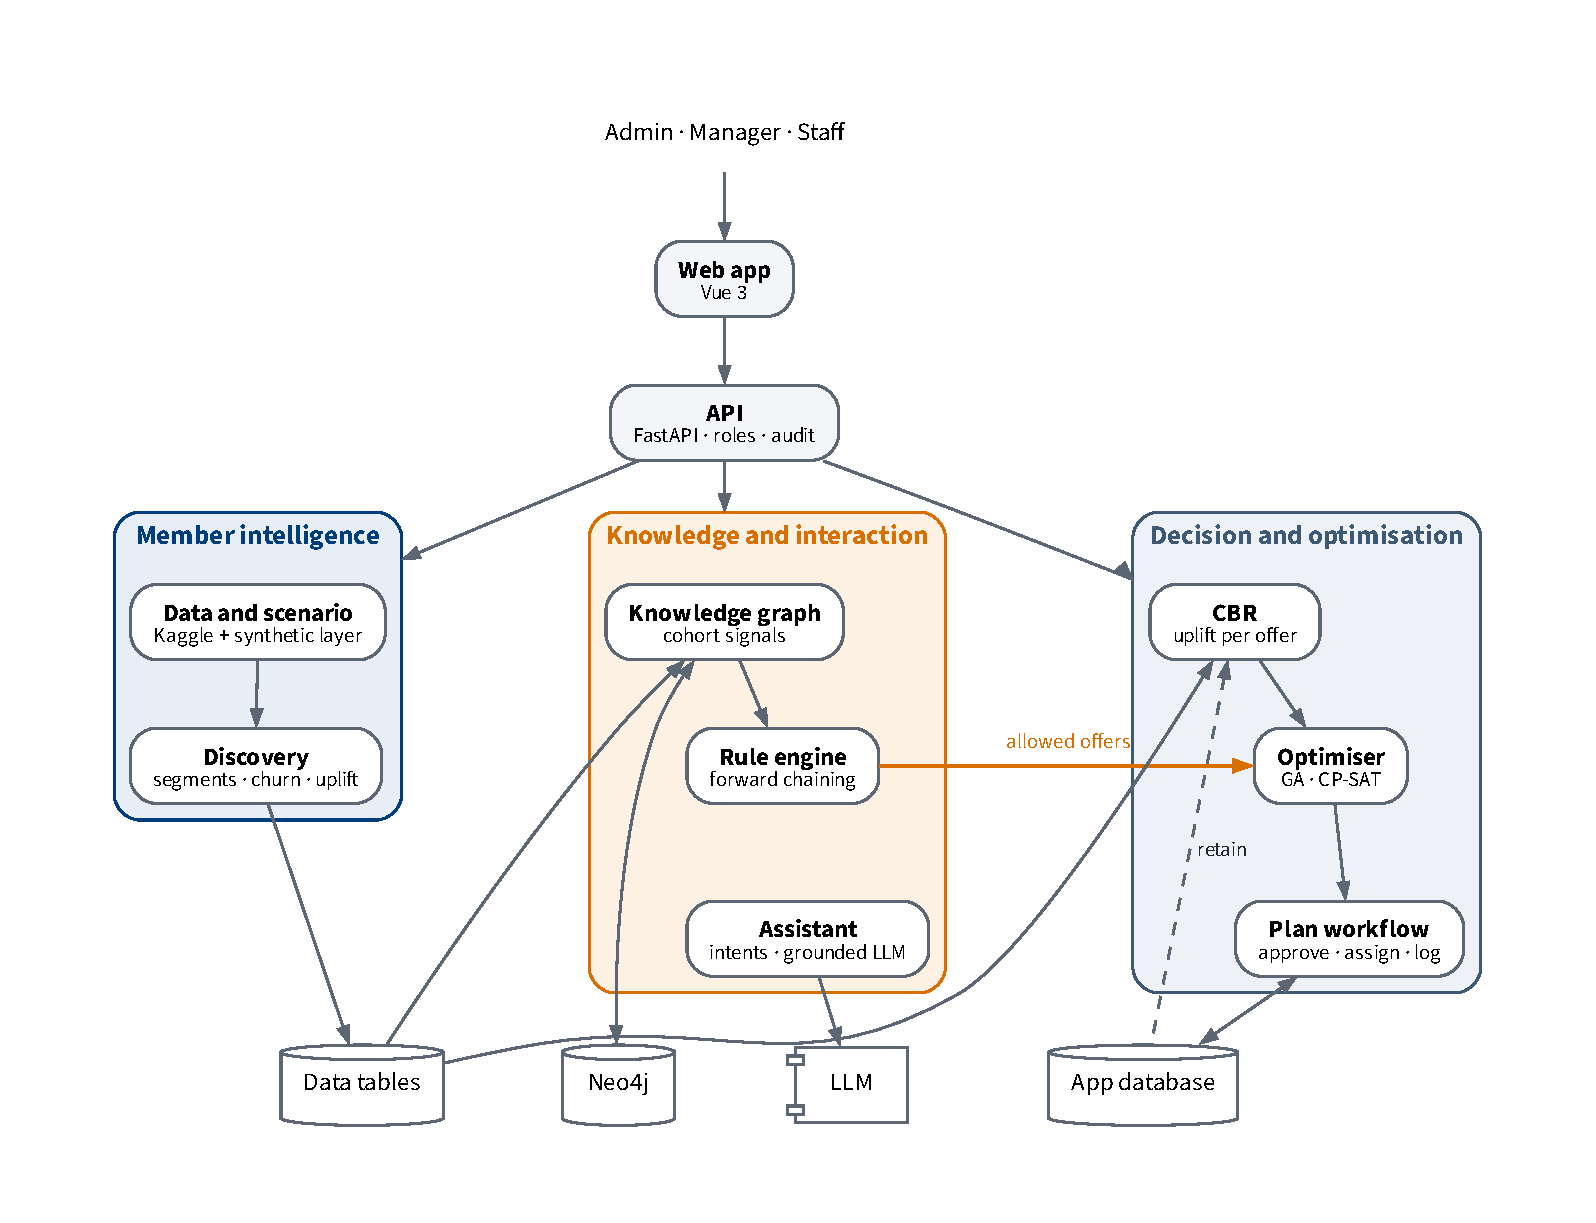
\includegraphics[width=0.74\linewidth]{diagrams/architecture.pdf}
  \caption{Architecture. Arrows show data flow; the dashed arrow is the learning loop through which logged outcomes return to the case base.}
  \label{fig:architecture}
\end{figure}

\begin{figure}[!htb]
  \centering
  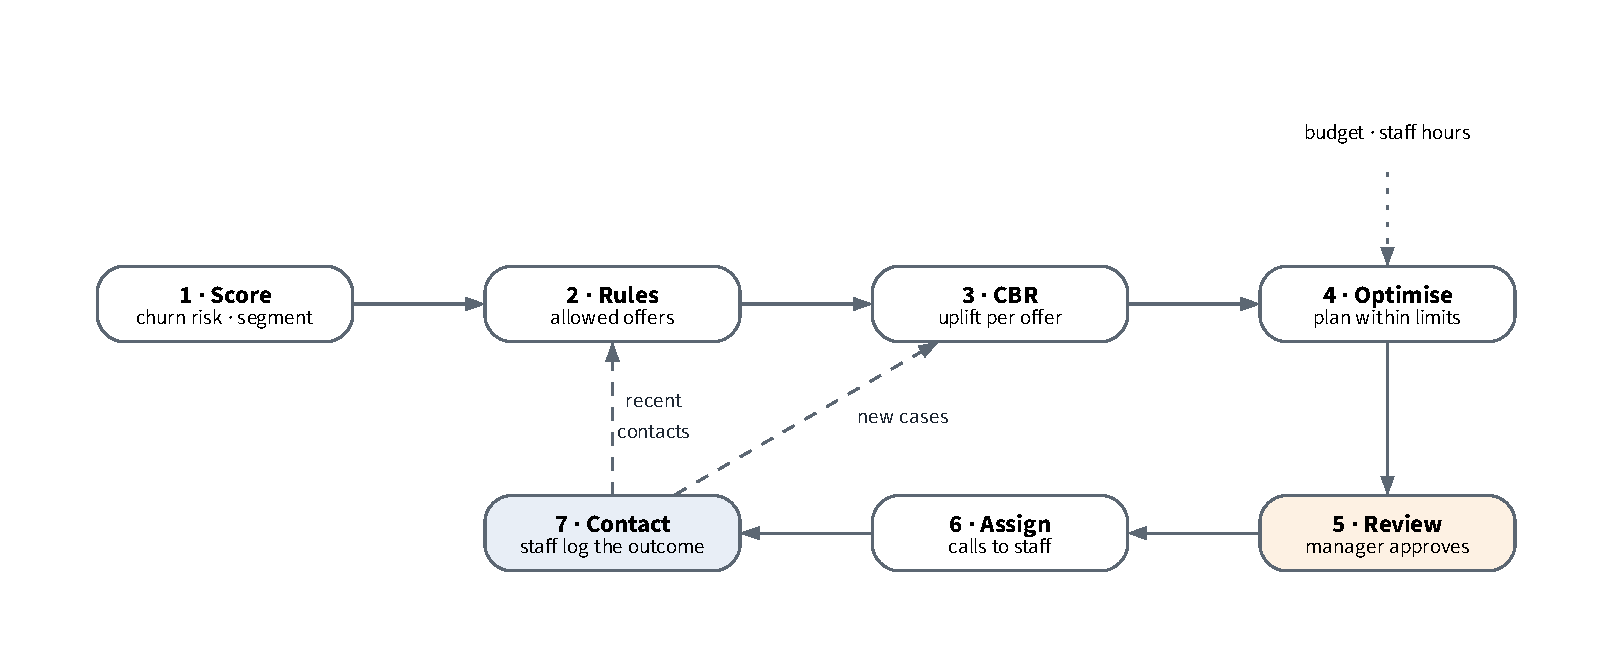
\includegraphics[width=0.92\linewidth]{diagrams/weekly-flow.pdf}
  \caption{The weekly cycle: steps 1--4 run automatically within the week's budget and staff hours; the manager reviews and approves, and staff contact members and log outcomes.}
  \label{fig:weekly}
\end{figure}

\section{Data and the scenario layer}
\label{sec:data}

Segmentation and churn prediction use only the 4,000 real members of the public \emph{Gym Customers Features and Churn} dataset~\cite{vinueza-gym}: 14 columns, 26.5\% churners, split 3,200/800 with stratification, and four derived features such as the visit trend (this month's visits over the lifetime rate), whose median is 0.69 for members who left and 1.00 for those who stayed (\cref{fig:trend}). Two same-month columns may leak the label, so E2 reports the model with and without them. The snapshot has no clubs, classes, offers or contact history, so a documented \emph{scenario layer} attaches a synthetic gym: three clubs, nine instructors and 18 classes consistent with each member's real visits; four offers with costs, staff minutes and stock; a heterogeneous ground-truth uplift for all 16,000 member--offer pairs (mean +5.8 points); two gym events (an instructor leaving and a class cancelled); and a randomised history of 2,400 past contacts (\cref{fig:scenario}). The ground truth is used only to grade, never by an estimator or planner. One command rebuilds every table, model and score in about 20 seconds from one seed.

\begin{figure}[!htb]
  \centering
  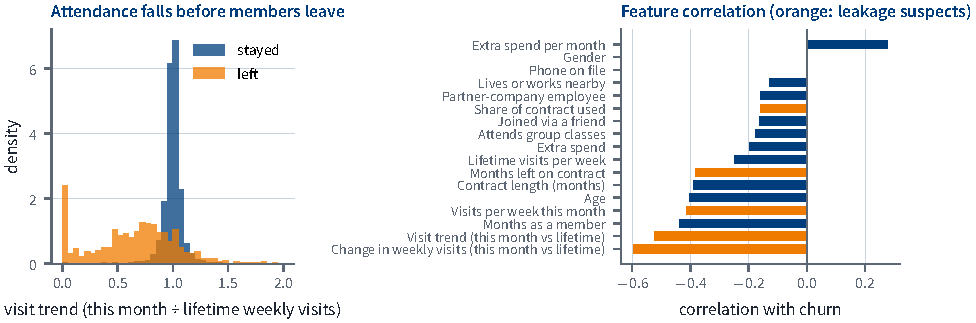
\includegraphics[width=\linewidth]{generated/trend_correlation.pdf}
  \caption{Left: the visit trend of members who stayed clusters at 1, while members who left spread below it, with a spike at 0 for those who did not come this month (medians 1.00 and 0.69). Right: correlation of each feature with churn; the two strongest are leakage suspects. Real Kaggle data.}
  \label{fig:trend}
  \source{\code{scripts/figures.py} (\code{trend}), as in \code{a_features_leakage.ipynb}, cells 2--4.}
\end{figure}
\begin{figure}[!htb]
  \centering
  \pgfplotstableread{\results{a5_true_uplift_by_segment.csv}}\upseg
  \begin{tikzpicture}
    \begin{axis}[anchorhbar, scale only axis, width=0.33\linewidth, height=4.4cm, bar width=3.6pt,
        ytick=data, yticklabels from table={\upseg}{segment}, y dir=reverse,
        enlarge y limits=0.16, xlabel={true uplift (percentage points)}, xmin=-5, xmax=26,
        legend style={at={(0.5,1.03)}, anchor=south, legend columns=2, /tikz/every even column/.append style={column sep=6pt}}, reverse legend,
        title={Effect by segment and offer}, title style={yshift=13mm}]
      \addplot[fill=cSky]    table[y expr=\coordindex, x expr=\thisrow{checkin_message}*100]{\upseg};
      \addplot[fill=cTeal]   table[y expr=\coordindex, x expr=\thisrow{class_pass}*100]{\upseg};
      \addplot[fill=cOrange] table[y expr=\coordindex, x expr=\thisrow{discount_1m}*100]{\upseg};
      \addplot[fill=cBlue]   table[y expr=\coordindex, x expr=\thisrow{free_pt_session}*100]{\upseg};
      \legend{Check-in message, Class pass, 20\% discount, Free PT session}
    \end{axis}
  \end{tikzpicture}\hfill
  \begin{tikzpicture}
    \begin{axis}[anchorhbar, scale only axis, width=0.24\linewidth, height=4.4cm, bar width=7pt, bar shift=0pt,
        symbolic y coords={All treated,Free PT session,Class pass,20\% discount,Check-in message,No contact},
        ytick={All treated,Free PT session,Class pass,20\% discount,Check-in message,No contact},
        y dir=reverse, enlarge y limits=0.11, xmin=60, xmax=80, xlabel={members who stayed (\%)},
        title={Intervention history}, title style={yshift=13mm}, clip=false,
        nodes near coords={\axisnum{\pgfplotspointmeta}}, nodes near coords style={font=\sffamily\scriptsize, text=navy},
        every node near coord/.append style={/pgf/number format/.cd, fixed, fixed zerofill, precision=1}]
      \addplot[fill=cGrey] coordinates {(67.0,No contact)};
      \addplot[fill=cBlue] coordinates {(67.8,Check-in message) (71.0,20\% discount) (71.2,Class pass) (77.6,Free PT session)};
      \addplot[fill=navy]  coordinates {(71.9,All treated)};
      \draw[cGrey, dashed, line width=0.6pt] (axis cs:67.0,No contact) -- (axis cs:67.0,All treated);
    \end{axis}
  \end{tikzpicture}
  \caption{The scenario's ground truth. Left: mean true uplift by segment and offer; a discount backfires on annual members. Right: share who stayed in each arm of the randomised history against the 984 controls (dashed).}
  \label{fig:scenario}
  \source{\code{results/a5_true_uplift_by_segment.csv}; \code{a_scenario_uplift.ipynb}.}
\end{figure}

\section{Methods}
\label{sec:methods}

\subsection{Member intelligence}

K-means~\cite{arthur2007kmeanspp} on seven behavioural features gives segments that staff can name; $k$ is chosen by a fixed rule on the silhouette~\cite{rousseeuw1987silhouettes} and names come from rules on the centres, so they survive a rebuild. Churn is predicted by the mean of a class-weighted logistic regression and LightGBM~\cite{ke2017lightgbm} over 17 features (\cref{fig:churnpipe}). Class weights matched SMOTE-NC~\cite{chawla2002smote} in cross-validation and were kept as simpler; a Platt calibrator~\cite{platt1999probabilistic} fitted on a held-out slice makes the probabilities honest, which matters because the planner multiplies them by uplift and value. Training members are scored out of fold, and each member's five drivers average the logistic-regression term with LightGBM's TreeSHAP value~\cite{lundberg2020trees} (\cref{fig:shap}). A T-learner~\cite{kunzel2019metalearners}, one outcome model per offer and one for controls, is the uplift benchmark.

\begin{figure}[!htb]
  \centering
  \begin{tikzpicture}[font=\sffamily\scriptsize,
      box/.style={draw=nusBlue, line width=0.6pt, rounded corners=2pt, fill=tint, align=center, minimum height=11mm, text width=23mm, text=ink},
      key/.style={box, fill=nusBlue, text=white, font=\sffamily\bfseries\scriptsize},
      outbox/.style={box, draw=nusOrange, fill=tintOrange},
      arr/.style={-{Latex[length=1.8mm]}, draw=muted, line width=0.6pt}]
    \node[box]    (f)    at (0,0)       {17 features\\13 Kaggle + 4 derived};
    \node[box]    (lr)   at (31mm,7.5mm)  {logistic regression\\class-weighted};
    \node[box]    (gb)   at (31mm,-7.5mm) {LightGBM\\300 trees, 15 leaves};
    \node[key]    (m)    at (62mm,0)    {mean of the two\\probabilities};
    \node[key]    (pl)   at (93mm,0)    {Platt calibration\\(640-member slice)};
    \node[outbox] (band) at (124mm,7.5mm)  {risk band\\high · medium · low};
    \node[outbox] (drv)  at (124mm,-7.5mm) {five drivers\\LR term + TreeSHAP};
    \coordinate (fs) at ($(f.east)!0.5!(lr.west|-f.east)$);
    \draw[arr] (f.east) -- (fs) |- (lr.west);
    \draw[arr] (fs) |- (gb.west);
    \coordinate (ms) at ($(lr.east|-m.west)!0.5!(m.west)$);
    \draw[draw=muted, line width=0.6pt] (lr.east) -| (ms);
    \draw[draw=muted, line width=0.6pt] (gb.east) -| (ms);
    \draw[arr] (ms) -- (m.west);
    \draw[arr] (m) -- (pl);
    \coordinate (ps) at ($(pl.east)!0.5!(band.west|-pl.east)$);
    \draw[draw=muted, line width=0.6pt] (pl.east) -- (ps);
    \draw[arr] (ps) |- (band.west);
    \draw[arr] (ps) |- (drv.west);
  \end{tikzpicture}
  \caption{The churn pipeline, fitted on 2,560 training members and calibrated on the remaining 640.}
  \label{fig:churnpipe}
\end{figure}

\begin{figure}[!htb]
  \centering
  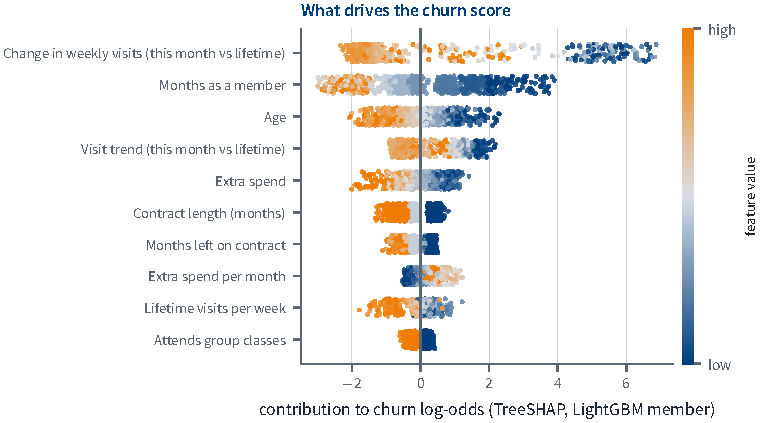
\includegraphics[width=0.66\linewidth]{generated/shap.pdf}
  \caption{TreeSHAP values of the LightGBM member on the 800 test members, for the ten most influential features. Each dot is a member, coloured by its feature value; dots to the right push towards churn. Real Kaggle data.}
  \label{fig:shap}
  \source{\code{scripts/figures.py} (\code{churn}), as in \code{a_churn.ipynb}, cell 5.}
\end{figure}
\subsection{Decision automation}
\label{sec:acquisition}

A forward-chaining engine~\cite{russell2021aima} runs 29 YAML rules: 8 \emph{derive} rules name patterns (falling regular, new member, routine disrupted), 16 \emph{playbooks} propose an offer on a channel, with twins for members without a phone, and 5 \emph{guardrails} block offers (contact and offer caps, eligibility, no paid offers at low risk, no repeat training session). Conflicts resolve by salience, specificity and order; each rule fires once, and blocks are applied after the loop, so guardrails always win. Every rule cites its source, a validator rejects inconsistent rule bases, and administrators edit, test, version and roll back rules in the application. Thresholds were drafted on the training data and adjusted after three \emph{simulated} manager interviews, which are disclosed as plausible opinion, not evidence.

\subsection{Decision and optimisation}

Each allowed member--offer--channel option is valued as $v_{mo} = \hat u_{mo} f_m H - c_o$, the estimated uplift~\cite{radcliffe2007uplift} times the monthly fee over a cautious six-month horizon, minus the offer's cost. The uplift comes from case-based reasoning~\cite{aamodt1994cbr} (\cref{fig:cbr}): retrieve the 200 nearest past cases in one shared neighbourhood of treated and untreated members, reuse it as a local A/B test, revise by empirical-Bayes shrinkage towards the offer's average~\cite{efron1975stein}, and retain logged outcomes as evidence but never in the averages, because the planner's own choices would bias them. A null test with shuffled offers rejected an earlier design that measured risk instead of effect. The plan maximises total value within budget, staff minutes, trainer minutes and stock, plus two effects between members who train together: \emph{spillover} and \emph{diminishing returns} per instructor. These make the problem non-linear, so a genetic algorithm (DEAP~\cite{fortin2012deap}) searches it with a repair operator and a greedy seed, while CP-SAT~\cite{ortools} solves the linear case exactly and benchmarks the full one on small instances. A policy evaluator grades plans against the true effects and is never used to choose one.

\begin{figure}[!htb]
  \centering
  % The case-based reasoner as a retrieve-reuse-revise-retain cycle; shared by both reports.
\begin{tikzpicture}[font=\sffamily\scriptsize,
    stage/.style={rectangle split, rectangle split parts=2, rectangle split part fill={nusBlue, white},
      draw=nusBlue, line width=0.6pt, text width=41mm, align=left, inner xsep=5pt, inner ysep=3.2pt,
      execute at begin node={\lefthyphenmin=64 \righthyphenmin=64 }},
    cyc/.style={-{Stealth[length=2.6mm, width=2.2mm]}, draw=nusOrange, line width=1.3pt},
    io/.style={-{Stealth[length=2.2mm, width=1.8mm]}, draw=muted, line width=0.7pt},
    iolab/.style={font=\sffamily\scriptsize, text=muted, align=center},
    link/.style={-{Stealth[length=1.8mm, width=1.5mm]}, draw=nusOrange!75, line width=0.7pt, dash pattern=on 2.2pt off 1.6pt},
    linklab/.style={font=\sffamily\tiny, text=nusOrange!85!black, fill=white, inner sep=1pt}]
  \newcommand{\stephead}[2]{\textcolor{white}{\bfseries\small #1\enskip #2}}
  \node[stage] (ret) at (-34mm, 19mm) {\stephead{1}{Retrieve}\nodepart{two}\color{ink}the 200 nearest past cases on 17 features, in one shared neighbourhood of treated and untreated members};
  \node[stage] (reu) at ( 34mm, 19mm) {\stephead{2}{Reuse}\nodepart{two}\color{ink}a local A/B test: the kernel-weighted stay rate with the offer minus the rate without it};
  \node[stage] (rev) at ( 34mm,-19mm) {\stephead{3}{Revise}\nodepart{two}\color{ink}empirical-Bayes shrinkage of the noisy local estimate towards the offer's average effect};
  \node[stage] (rtn) at (-34mm,-19mm) {\stephead{4}{Retain}\nodepart{two}\color{ink}each logged outcome becomes a new case, used as evidence but never in the offer averages};
  \node[circle, draw=nusOrange, line width=1pt, fill=tintOrange, minimum size=19mm, inner sep=0pt, align=center, text=ink] (cb) at (0,0)
    {\bfseries\small Case base\\[2pt]\mdseries\tiny 2,400 randomised\\[-1pt]\tiny cases + outcomes};
  \draw[cyc] (ret.east) -- (reu.west);
  \draw[cyc] (reu.south) -- (rev.north);
  \draw[cyc] (rev.west) -- (rtn.east);
  \draw[cyc] (rtn.north) -- (ret.south);
  \draw[link] (cb.135) -- node[linklab, sloped] {read} (ret.south east);
  \draw[link] (rtn.north east) -- node[linklab, sloped] {write} (cb.225);
  \draw[io] ([xshift=-16mm]ret.west) -- node[iolab, above=1pt] {member\\and offer} (ret.west);
  \draw[io] ([xshift=-16mm]rtn.west) -- node[iolab, above=1pt] {outcome\\logged} (rtn.west);
  \draw[io] (rev.east) -- node[iolab, above=1pt] {estimate +\\precedents} ([xshift=16mm]rev.east);
\end{tikzpicture}

  \caption{The case-based reasoner. The neighbours that produce an estimate are shown to staff as its precedents.}
  \label{fig:cbr}
\end{figure}

\subsection{Knowledge graph and staff assistant}

A Neo4j knowledge graph~\cite{hogan2021kg} links members, classes, instructors, clubs, offers and events through read-only parameterised Cypher. It flags members whose anchor instructor left or whose class was cancelled, as rule facts cached so the rules work without Neo4j; it gives the optimiser its class cohorts; and it simulates an event's impact without changing data (\cref{fig:kgsim}). The staff assistant routes a question to one of seven intents with sentence-embedding centroids~\cite{reimers2019sbert} and an \enquote{unknown} threshold, fills slots, runs one deterministic tool, and lets the language model only phrase the numbered evidence with citations, or answer that it does not know (\cref{fig:assistantpipe,fig:assistant}). Without the model, it returns the cited evidence itself.

\begin{figure}[!htb]
  \centering
  \begin{tikzpicture}[font=\sffamily\scriptsize,
      st/.style={draw=nusBlue, line width=0.6pt, rounded corners=2pt, fill=tint, align=center, minimum height=11mm, text width=21mm, text=ink},
      llm/.style={st, draw=nusOrange, fill=tintOrange},
      arr/.style={-{Latex[length=1.8mm]}, draw=muted, line width=0.6pt}]
    \node[st]  (q)  at (0,0)        {\textbf{question}\\+ member on page};
    \node[st]  (i)  at (26.5mm,0)   {\textbf{intent}\\embedding centroid, threshold 0.35};
    \node[st]  (s)  at (53mm,0)     {\textbf{slots}\\ids, amounts, names, filters};
    \node[st]  (t)  at (79.5mm,0)   {\textbf{tool}\\one deterministic function per intent};
    \node[st]  (e)  at (106mm,0)    {\textbf{evidence}\\numbered lines [E1], [E2]…};
    \node[llm] (l)  at (132.5mm,0)  {\textbf{LLM}\\phrases and cites, or says it does not know};
    \foreach \a/\b in {q/i, i/s, s/t, t/e, e/l} \draw[arr] (\a) -- (\b);
  \end{tikzpicture}
  \caption{The assistant pipeline: the language model never chooses a tool and never sees data a tool did not return.}
  \label{fig:assistantpipe}
\end{figure}

\begin{figure}[!htb]
  \centering
  \begin{subfigure}[t]{0.495\linewidth}
    \screenshot[\linewidth]{screens/graph-content.png}
    \caption{Simulating instructor Maya Chen leaving: 312 members affected, 54 at high risk, with her neighbourhood.}
    \label{fig:kgsim}
  \end{subfigure}\hfill
  \begin{subfigure}[t]{0.495\linewidth}
    \screenshot[\linewidth]{screens/assistant-content.png}
    \caption{The assistant answering about member M1460 with the local \code{qwen2.5:7b-instruct} model, citing its sources.}
    \label{fig:assistant}
  \end{subfigure}
  \caption{The knowledge graph and the staff assistant in the application.}
\end{figure}
\section{System development and implementation}
\label{sec:impl}

One command builds the data and models, migrates and seeds the database with a demo week, and loads the graph. Sixteen pages serve three roles (\cref{fig:screens}): managers work from the dashboard, plan and scenarios; staff from a call sheet with talking points, message drafts and two-tap outcome logging; administrators from versioned rules, offers, data and models, users and an audit log of every write. Member~360 shows every component's reasoning about one member on one screen. Risk is always shown as text and colour; planning continues when Neo4j or the language model is down; and 195 offline tests guard against leakage, infeasible plans, rule order, unsafe queries and role or audit errors.

\begin{figure}[!htb]
  \centering
  \screenshot[\linewidth]{screens/dashboard.png}\par\medskip
  \begin{subfigure}[t]{0.495\linewidth}
    \screenshot[\linewidth]{screens/member360-content.png}
    \caption{Member 360: risk, drivers, profile and rule trace for one member.}
  \end{subfigure}\hfill
  \begin{subfigure}[t]{0.495\linewidth}
    \screenshot[\linewidth]{screens/plan-content.png}
    \caption{The weekly plan: 182 approved contacts, each with a reason.}
  \end{subfigure}
  \caption{The application on the demo data. Top: the manager's dashboard.}
  \label{fig:screens}
\end{figure}

\FloatBarrier
\section{Experiments and findings}
\label{sec:exp}

Eight experiments test the objectives. E1 and E2 use only the 4,000 real members. E3--E7 are graded against the scenario layer's ground truth, which no estimator or planner ever reads, so they show that the system recovers effects of this kind, not how large real effects are. E8 evaluates the assistant on the system's own evidence (\cref{tab:exp}). Every number below comes from a committed results file or notebook, all reproducible from seed 42.

\begin{table}[!htb]
  \caption{The eight experiments: real-data experiments use the 4,000 Kaggle members; scenario experiments are graded against the synthetic ground truth.}
  \label{tab:exp}
  \begin{tabularx}{\linewidth}{@{}l L L l@{}}
    \toprule
    & \hd{Question} & \hd{Key result} & \hd{Verdict} \\
    \midrule
    E1 & meaningful segments? \databadge{real} & $k=4$ by rule; stability ARI 1.00; churn from 94.6\% to 1.4\% & \verdict{met} \\
    E2 & churn model beats simple rules? \databadge{real} & F1 0.908, PR-AUC 0.973, Brier 0.035 vs 0.862 / 0.953 / 0.056 (logistic) and 0.549 / 0.390 / 0.336 (visit rule) & \verdict{met} \\
    E3 & who is persuadable? \databadge{scenario} & CBR ties the T-learner (Spearman 0.39 each), better for PT and discount & \verdict{partly} \\
    E4 & more members per dollar? \databadge{scenario} & 22--138\% more members kept than by risk or schedule; 0 of 198 plans infeasible & \verdict{met} \\
    E5 & GA good and fast enough? \databadge{scenario} & within 0.24\% of the optimum on small instances; 33\,s for 2,000 members & \verdict{partly} \\
    E6 & rules correct; guardrails matter? \databadge{scenario} & 0 validator issues; 29 of 29 cases; guardrails remove 31.3\% of proposals & \verdict{met} \\
    E7 & graph signals add information? \databadge{scenario} & no ranking gain; 243 extra low-risk members reached; +7 members at 120\,h & \verdict{partly} \\
    E8 & assistant accurate, grounded? \databadge{scenario} & 96.2\% of sentences supported; held-out routing 50.0\% vs 54.2\% for keywords & \verdict{partly} \\
    \bottomrule
  \end{tabularx}
  \source{\code{SystemCode/notebooks/results/}; method, baseline and caveats for each experiment follow.}
\end{table}

\subsection{E1: Are the segments meaningful?}
\label{sec:e1}
\databadge{real}\quad\textsf{\small Baseline: every $k$ from 2 to 10}

K-means was fitted on the 3,200 training members for each $k$ and scored by silhouette, by stability across five other seeds (adjusted Rand index) and by how sharply the segments separate churn, which the clustering never sees.

\begin{figure}[!htb]
  \centering
  \pgfplotstableread{\results{e1_silhouette_by_k.csv}}\sil
  \pgfplotstableread{\results{e1_segment_profiles.csv}}\seg
  \begin{tikzpicture}
    \begin{axis}[anchor, scale only axis, width=0.36\linewidth, height=4.1cm, xlabel={number of segments \textit{k}},
        ylabel={silhouette}, ymin=0.15, ymax=0.182, xtick={2,...,10}, title={Silhouette on the training split},
        yticklabel style={/pgf/number format/fixed, /pgf/number format/precision=3}]
      \fill[nusOrange!12] (axis cs:3,0.1688) rectangle (axis cs:8,0.1776);
      \addplot[cBlue, mark=*, mark size=1.6pt] table[x index=0, y=silhouette]{\sil};
      \draw[nusOrange, dashed, line width=0.8pt] (axis cs:4,0.15) -- (axis cs:4,0.182);
      \node[font=\sffamily\tiny, text=nusOrange, anchor=south west] at (axis cs:4.1,0.151) {chosen \textit{k} = 4};
    \end{axis}
  \end{tikzpicture}\hfill
  \begin{tikzpicture}
    \begin{axis}[anchorhbar, scale only axis, width=0.3\linewidth, height=4.1cm, bar width=9pt,
        ytick=data, yticklabels from table={\seg}{name}, y dir=reverse, enlarge y limits=0.18,
        xmin=0, xmax=100, xlabel={churn rate (\%)}, title={Churn by segment (size)},
        nodes near coords={\axisnum[fixed, precision=1]{\pgfplotspointmeta}\,\%},
        nodes near coords style={font=\sffamily\scriptsize, text=ink}, point meta=x]
      \addplot[fill=cBlue] table[y expr=\coordindex, x expr=\thisrow{churn_rate}*100]{\seg};
    \end{axis}
  \end{tikzpicture}
  \caption{E1. Left: silhouette is low and nearly flat; the shaded band is within 5\% of the best $k$ between 3 and 8, and the rule picks the most detailed $k$ inside it. Right: the four segments separate churn from 94.6\% to 1.4\% (sizes 728, 1,365, 961 and 946).}
  \label{fig:e1}
  \source{\code{results/e1_silhouette_by_k.csv}, \code{results/e1_segment_profiles.csv}; \code{a_segmentation.ipynb}.}
\end{figure}

\paragraph{Results.} The documented rule chooses $k = 4$ (silhouette 0.174 against the best of 0.178 at $k = 3$); $k = 4$ adds a distinct annual-contract segment. Stability is very high: the mean adjusted Rand index across seeds is 1.00 (minimum 0.998). Test members fall into the segments in proportions within 4.2 percentage points of the training split, and churn separates by a factor of almost 70 (\cref{fig:e1}). The 728 \enquote{new and slipping} members hold about two-thirds of all churners.

\paragraph{Verdict} \verdict{met}. The segments are not geometrically crisp, as expected for behavioural data, but they are chosen by rule, stable, carry over to unseen members and separate risk in terms staff can name.

\subsection{E2: Does the churn model beat simple rules?}
\label{sec:e2}
\databadge{real}\quad\textsf{\small Baselines: a visit-threshold rule; a single logistic regression}

All metrics are on the 800 untouched test members, with churn as the positive class. A model that beats the baselines should do so on all three of F1 (the yes-or-no flag), PR-AUC (the ranking, suited to an imbalanced label~\cite{saito2015prc}) and the Brier score~\cite{brier1950verification} (the probabilities the planner consumes).

\begin{figure}[!htb]
  \centering
  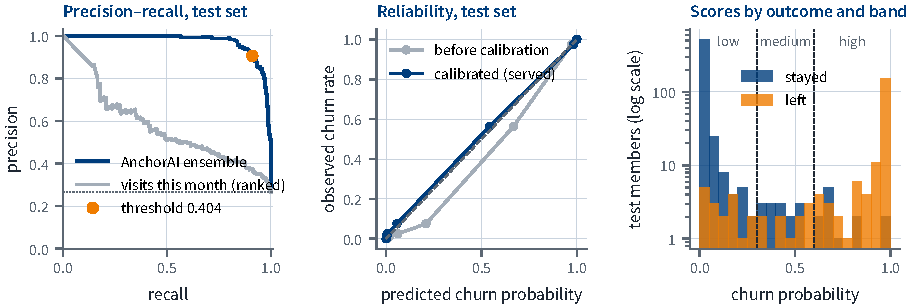
\includegraphics[width=\linewidth]{generated/churn_evaluation.pdf}
  \caption{E2 on the test set. Left: precision--recall of the ensemble against members ranked by this month's visits, with the operating point at the threshold 0.404. Centre: reliability before and after Platt calibration. Right: scores by actual outcome, with the band cut-offs at 0.3 and 0.6.}
  \label{fig:e2}
  \source{\code{scripts/figures.py} (\code{churn}), as in \code{a_churn.ipynb}, cells 3--4.}
\end{figure}

\begin{table}[!htb]
  \caption{E2. Test-set performance. The visit rule flags members with at most 1.63 visits a week this month, a threshold chosen on the training split.}
  \label{tab:e2}
  \begin{tabular*}{\linewidth}{@{\extracolsep{\fill}}l S[table-format=1.3] S[table-format=1.3] S[table-format=1.3] S[table-format=1.3] S[table-format=1.3] S[table-format=1.3]@{}}
    \toprule
    \hd{Model} & {\hd{F1}} & {\hd{Precision}} & {\hd{Recall}} & {\hd{PR-AUC}} & {\hd{ROC-AUC}} & {\hd{Brier}} \\
    \midrule
    AnchorAI ensemble, calibrated & \bfseries 0.908 & \bfseries 0.906 & \bfseries 0.910 & \bfseries 0.973 & \bfseries 0.988 & \bfseries 0.035 \\
    Single logistic regression & 0.862 & 0.818 & 0.910 & 0.953 & 0.978 & 0.056 \\
    Visit rule & 0.549 & 0.426 & 0.774 & 0.390 & 0.699 & 0.336 \\
    \midrule
    Ensemble without the five suspect features & 0.817 & & & 0.900 & & 0.069 \\
    \bottomrule
  \end{tabular*}
  \source{\code{results/e2_model_vs_baselines.csv}, \code{results/a_leakage.csv}.}
\end{table}

\paragraph{Results.} The ensemble beats both baselines on every metric (\cref{tab:e2}). At the threshold of 0.404 it flags 193 of the 212 test churners with 20 false alarms: about one flag in eleven is a member who stayed. Calibration moves the curve onto the diagonal (\cref{fig:e2}), so each band churns at about its predicted rate: high-band members churn at 93.9\% against 95.1\% predicted, medium at 41.7\% against 44.1\%, low at 2.9\% against 1.6\%. Without the suspect same-month columns, F1 falls to 0.817, the honest lower bound if those columns were recorded after the churn month. Recall is 0.985, 0.943 and 0.522 for ages 18--25, 26--30 and 31+: the model misses about half of the rare churners aged 31 and over (23 in the test set); we report this rather than hide it, and suggest staff review medium-risk members of that group.

\paragraph{Verdict} \verdict{met}. F1 0.908, PR-AUC 0.973 and Brier 0.035 against 0.862, 0.953 and 0.056 for logistic regression and 0.549, 0.390 and 0.336 for the visit rule, with calibrated probabilities the planner can use at face value.

\subsection{E3: Can we find who is persuadable?}
\label{sec:e3}
\databadge{scenario}\quad\textsf{\small Baselines: T-learner; churn risk used as uplift; random}

Estimates for all 16,000 member--offer pairs were compared with the true uplift by rank correlation and by the mean true uplift of each method's top 10\% of pairs; the same estimates then drove the greedy planner, graded by the evaluator.

\begin{figure}[!htb]
  \centering
  \pgfplotstableread{\results{e3_uplift_vs_truth.csv}}\upl
  \begin{tikzpicture}
    \begin{axis}[anchorbar, scale only axis, width=0.5\linewidth, height=4.2cm, bar width=5.5pt,
        ymin=-0.05, ymax=1, ylabel={Spearman with true uplift},
        xtick={0,...,4}, xticklabels={Check-in, Class pass, Discount, Free PT, All pairs},
        unbounded coords=discard, title={Ranking quality by offer}, title style={yshift=11pt}, enlarge x limits=0.13, ytick={0,0.25,...,1},
        legend style={at={(0.5,1.02)}, anchor=south, legend columns=4, /tikz/every even column/.append style={column sep=5pt}}]
      \addplot[fill=cBlue]   table[x expr=\coordindex,    y=spearman, skip coords between index={5}{20}]{\upl};
      \addplot[fill=cOrange] table[x expr=\coordindex-5,  y=spearman, skip coords between index={0}{5}, skip coords between index={10}{20}]{\upl};
      \addplot[fill=cSky]    table[x expr=\coordindex-10, y=spearman, skip coords between index={0}{10}, skip coords between index={15}{20}]{\upl};
      \addplot[fill=cGrey]   table[x expr=\coordindex-15, y=spearman, skip coords between index={0}{15}]{\upl};
      \legend{CBR, T-learner, churn risk, random}
    \end{axis}
  \end{tikzpicture}\hfill
  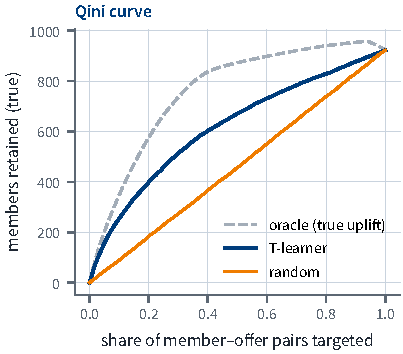
\includegraphics[width=0.4\linewidth]{generated/qini.pdf}
  \caption{E3. Left: rank correlation between estimated and true uplift; CBR gives every member the offer's average for the check-in and the class pass, so it has no ranking there. Right: Qini curve of the T-learner against the oracle and random targeting.}
  \label{fig:e3}
  \source{\code{results/e3_uplift_vs_truth.csv}, \code{results/a6_tlearner_recovery.csv}; \code{b_cbr.ipynb}, \code{a_scenario_uplift.ipynb}.}
\end{figure}

\paragraph{Results.} CBR ties the T-learner overall (Spearman 0.39 each), is better for the two large-effect offers (free PT 0.64 against 0.61; discount 0.48 against 0.27) and picks the pairs with the highest true effect (top-decile mean 0.177 against 0.159). It cannot separate members for the check-in and the class pass, whose effects of a few points are smaller than the noise in about 350 randomised cases per offer, so shrinkage honestly returns the average. Churn risk ranks well \emph{within} an offer, because scenario effects grow with risk, but says nothing about \emph{which} offer helps, so its top picks are weaker (0.125). Plans built on the estimates (\cref{tab:e4}) favour the T-learner at the default 36 staff hours, where cheap check-ins dominate and CBR cannot rank them, and CBR with more staff time. A null test with shuffled offers confirms that CBR does not invent effects.

\paragraph{Verdict} \verdict{partly}. CBR matches the T-learner overall, is better where effects are large and explains each estimate with real precedents; it is weaker where effects are small and staff time is scarce, which costs 3.7 retained members a week at the default settings. The team kept CBR as the planner's estimator for its inspectable precedents, with the T-learner as its benchmark.

\subsection{E4: Does AnchorAI retain more members per dollar?}
\label{sec:e4}
\databadge{scenario}\quad\textsf{\small Baselines: contact-all; risk-top-$k$; greedy-uplift}

Every planner ran at 36, 72 and 120 staff hours and several budgets, the genetic algorithm with three seeds, and every plan was graded by the evaluator as extra members kept beyond the roughly 2,660 of 4,000 who would stay anyway. Variant (a) gives every planner the true effects, isolating search quality; variant (b) gives them the estimates, as in real use. None of the 198 plans broke a limit.

\begin{figure}[!htb]
  \centering
  \begin{tikzpicture}
    \begin{axis}[anchorbar, width=\linewidth, height=4.3cm, bar width=6.5pt,
        symbolic x coords={36 h \$1.5k, 72 h \$1.5k, 72 h \$4k, 120 h \$1.5k, 120 h \$4k}, xtick=data,
        ymin=0, ymax=80, ylabel={extra members kept}, enlarge x limits=0.1,
        legend style={at={(0.02,0.98)}, anchor=north west, legend columns=4, /tikz/every even column/.append style={column sep=6pt}},
        nodes near coords={\axisnum{\pgfplotspointmeta}}, nodes near coords style={font=\sffamily\tiny, text=ink, rotate=90, anchor=west},
        every node near coord/.append style={/pgf/number format/.cd, fixed, fixed zerofill, precision=1}]
      \addplot[fill=cGrey]   coordinates {(36 h \$1.5k,10.4) (72 h \$1.5k,20.1) (72 h \$4k,20.2) (120 h \$1.5k,20.1) (120 h \$4k,20.2)};
      \addplot[fill=cSky]    coordinates {(36 h \$1.5k,13.7) (72 h \$1.5k,21.0) (72 h \$4k,21.4) (120 h \$1.5k,21.0) (120 h \$4k,21.4)};
      \addplot[fill=cOrange] coordinates {(36 h \$1.5k,28.8) (72 h \$1.5k,44.5) (72 h \$4k,50.1) (120 h \$1.5k,47.6) (120 h \$4k,64.1)};
      \addplot[fill=cBlue]   coordinates {(36 h \$1.5k,32.5) (72 h \$1.5k,45.7) (72 h \$4k,54.0) (120 h \$1.5k,47.6) (120 h \$4k,70.8)};
      \legend{contact-all, risk-top-\textit{k}, greedy-uplift, genetic algorithm}
    \end{axis}
  \end{tikzpicture}
  \caption{E4 (a), perfect knowledge: extra members kept by each planner, by staff hours and weekly budget. Planning by effect keeps 1.9 to 3.5 times as many members as contacting by schedule or by risk. The estimates behind the system's own plans are in \cref{tab:e4}.}
  \label{fig:e4}
  \source{\code{results/e4_optimiser.csv}, mean over three seeds; \code{b_ga.ipynb}.}
\end{figure}

\begin{table}[!htb]
  \caption{E4 (b), estimated effects: extra members kept, as the system runs. Default configuration: the genetic algorithm on CBR estimates.}
  \label{tab:e4}
  \begin{tabular*}{\linewidth}{@{\extracolsep{\fill}}l S[table-format=2.1] S[table-format=2.1] S[table-format=2.1] S[table-format=2.1] S[table-format=2.1] S[table-format=2.1]@{}}
    \toprule
    & {\hd{Contact-}} & {\hd{Risk-}} & \multicolumn{2}{c}{\hd{CBR}} & \multicolumn{2}{c}{\hd{T-learner}} \\
    \cmidrule(lr){4-5}\cmidrule(l){6-7}
    \hd{Staff hours, budget} & {\hd{all}} & {\hd{top-$k$}} & {\hd{greedy}} & {\hd{GA}} & {\hd{greedy}} & {\hd{GA}} \\
    \midrule
    36 h, \$1,500 & 10.4 & 13.7 & 21.0 & 16.7 & 24.6 & \bfseries 24.9 \\
    72 h, \$1,500 & 20.1 & 21.0 & \bfseries 36.6 & 35.5 & 35.1 & 35.1 \\
    120 h, \$4,000 & 20.2 & 21.4 & \bfseries 51.9 & 48.1 & 50.7 & 50.7 \\
    \bottomrule
  \end{tabular*}
  \source{\code{results/e4_estimates.csv}, mean over seeds.}
\end{table}

\paragraph{Results.} With perfect knowledge the genetic algorithm beats greedy wherever two limits bind together and ties where one dominates (\cref{fig:e4}). On estimates (\cref{tab:e4}), every effect-based plan beats contacting by schedule or risk, and per staff hour at the default week the default configuration keeps 0.46 members against 0.29 for contact-all and 0.38 for risk-top-$k$. But the genetic algorithm's advantage reverses on noisy estimates: against greedy, its true net value ranges from +2.2\% to +9.2\% with perfect knowledge, $-1.5\%$ to $+0.4\%$ on the T-learner and $-33.8\%$ to $-1.0\%$ on CBR. This is the optimiser's curse~\cite{smith2006curse}: the harder a planner optimises noisy estimates, the more it selects the options whose estimates happen to be too high.

\paragraph{Verdict} \verdict{met}. Planning by estimated effect, as the system runs by default, keeps 22\% to 138\% more members than contacting by risk or schedule in every setting tested, without breaking a limit. The size of the gain depends on the estimates more than the optimiser: on today's CBR estimates, the simpler greedy planner, selectable on the same page, keeps more members than the default genetic algorithm.

\subsection{E5: How good and how fast is the genetic algorithm?}
\label{sec:e5}
\databadge{scenario}\quad\textsf{\small Benchmark: CP-SAT's proven optimum on the planner's objective}

The genetic algorithm was compared with CP-SAT on the planner's own objective: the linear objective on the full gym, and the full objective (with spillover and diminishing returns) on resampled instances small enough to prove optimality.

\begin{figure}[!htb]
  \centering
  \pgfplotstableread{\results{e5_speed.csv}}\spd
  \begin{tikzpicture}
    \begin{axis}[anchor, scale only axis, width=0.36\linewidth, height=4.1cm, ymode=log,
        xlabel={members with options}, ylabel={seconds (log scale)}, title={Run time by size},
        xtick={250,1000,2000,4000}, log basis y=10, ymin=0.08, ymax=150,
        yticklabel={\pgfmathparse{10^\tick}\axisnum[fixed, precision=1]{\pgfmathresult}},
        legend style={at={(0.98,0.03)}, anchor=south east}]
      \addplot[cBlue, mark=*, mark size=1.6pt] table[x=members, y=ga_seconds]{\spd};
      \addplot[cOrange, mark=square*, mark size=1.5pt] table[x=members, y=cp_sat_linear_seconds]{\spd};
      \addplot[only marks, mark=-, mark size=5pt, line width=1.2pt, color=ink] coordinates {(2000,30) (4000,60)};
      \legend{GA (300 generations), CP-SAT (linear), target}
    \end{axis}
  \end{tikzpicture}\hfill
  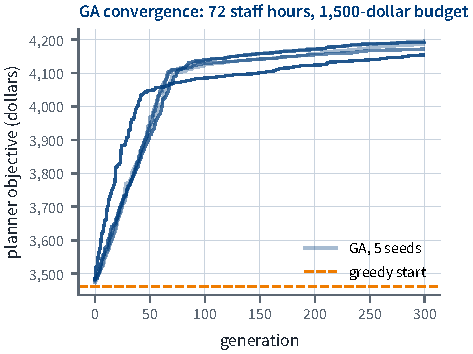
\includegraphics[width=0.48\linewidth]{generated/ga_convergence.pdf}
  \caption{E5. Left: run time grows about linearly; this run missed the 30\,s and 60\,s targets by about 10\%. Right: five seeds climb from the greedy start and plateau about 20\% above it (regenerated on the seeded database; the committed run's five seeds end within 0.2\% of each other).}
  \label{fig:e5}
  \source{\code{results/e5_speed.csv}; \code{scripts/figures.py} (\code{ga}), as in \code{b_exact.ipynb}.}
\end{figure}

\paragraph{Results.} On the linear objective, CP-SAT proves the optimum for the full gym in 1.2--1.4\,s; the genetic algorithm is within 0.8--2.3\% of it and greedy within 15--32\%. On the full objective, the genetic algorithm matches the proven optimum on 8 of 9 instances of 20--40 members and comes within 0.24\% at 50; at 200 members it beats CP-SAT's time-limited best by 1.0\%, though at 100 it is 2.5\% below. Greedy is 14--27\% below the optimum on average. Its advantage over greedy holds, at 16--26\%, for every combination of spillover $\beta \in \{0, 0.5, 1\}$ and diminishing returns $d \in \{0, 0.02, 0.05\}$. It takes 18\,s for 1,000 members and 33\,s for 2,000 (\cref{fig:e5}).

\paragraph{Verdict} \verdict{partly}. On the linear problem CP-SAT is the better tool, exact and faster. The genetic algorithm earns its place on the full objective at real size, where it is near-optimal and robust to the assumed effect strengths; its speed is at the edge of the targets.

\subsection{E6: Are the rules correct, and do guardrails matter?}
\label{sec:e6}
\databadge{scenario}\quad\textsf{\small Baseline: the same playbooks with guardrails switched off}

The full rule base ran on all 4,000 members with facts built exactly as the API builds them: the validator, the 29 hand-built cases, coverage, and 60 plans with and without guardrails, scored by the true uplift.

\begin{figure}[!htb]
  \centering
  \begin{tikzpicture}
    \begin{axis}[anchorhbar, scale only axis, width=0.42\linewidth, height=3.2cm, bar width=8pt,
        symbolic y coords={G05 PT eligibility,G04 low risk,G03 discount,G02 offer cap,G01 contact cap},
        ytick=data, xmin=0, xmax=1250, xlabel={proposals removed}, title={What the guardrails remove},
        nodes near coords={\axisnum{\pgfplotspointmeta}}, nodes near coords style={font=\sffamily\scriptsize, text=ink}]
      \addplot[fill=cBlue] coordinates {(1029,G01 contact cap) (0,G02 offer cap) (0,G03 discount) (7,G04 low risk) (44,G05 PT eligibility)};
    \end{axis}
  \end{tikzpicture}\hfill
  \begin{tikzpicture}
    \begin{axis}[anchorbar, scale only axis, width=0.34\linewidth, height=3.2cm, bar width=9pt,
        symbolic x coords={36 h,120 h}, xtick=data, ymin=0, ymax=62, ylabel={extra members kept}, enlarge x limits=0.5,
        title={Plan value, greedy, \$1,500}, legend style={at={(0.03,0.97)}, anchor=north west},
        nodes near coords={\axisnum{\pgfplotspointmeta}}, nodes near coords style={font=\sffamily\scriptsize, text=ink},
        every node near coord/.append style={/pgf/number format/.cd, fixed, fixed zerofill, precision=1}]
      \addplot[fill=cBlue]   coordinates {(36 h,16.539) (120 h,40.447)};
      \addplot[fill=cGrey]   coordinates {(36 h,17.638) (120 h,54.727)};
      \legend{with guardrails, without}
    \end{axis}
  \end{tikzpicture}
  \caption{E6. Left: of 3,448 proposals over 1,422 members, guardrails remove 1,080 (31.3\%), almost all of them contacts inside the 30-day cap. Right: their cost in plan value as the scenario measures it, which has no contact-fatigue effect and so cannot see what the cap protects against.}
  \label{fig:e6}
  \source{\code{results/e6_guardrail_bites.csv}, \code{results/e6_plan_value.csv}; \code{c_e6_rules.ipynb}.}
\end{figure}

\paragraph{Results.} The validator reports no issues, all 29 cases match, and every rule fires for at least one member. Guardrails remove 31.3\% of proposals (\cref{fig:e6}); every guardrail-free plan contacts members again within 30 days (75--148 times per plan at 36\,h), and no guarded plan contains a violation. The 386 members without a phone receive the email or in-person twin of each playbook, never an SMS or a call. At 36 staff hours, where staff time binds, removing the guardrails changes plan value by $-1.0$ to $+1.4$ members; at 120\,h the guardrail-free plans gain 6--14 members by re-contacting members inside the cap.

\paragraph{Verdict} \verdict{met}. The rule base is consistent and its guardrails do real work. Their cost is zero to small at the seeded staff level and up to about 14 members at 120\,h, but the scenario has no fatigue effect to price, so we claim safety and auditability, not a retention gain.

\subsection{E7: Do knowledge-graph signals add information?}
\label{sec:e7}
\databadge{scenario}\quad\textsf{\small Baseline: churn probability alone}

The graph's event flags were tested against the scenario's true post-event hazard (the Kaggle label knows nothing of the synthetic events): their lift, whether adding them to the churn ranking surfaces higher-hazard members among the 800 test members (1,000 bootstrap resamples), and their effect on rules and plans.

\begin{figure}[!htb]
  \centering
  \pgfplotstableread{\results{e7_ranking.csv}}\rk
  \begin{tikzpicture}
    \begin{axis}[anchor, scale only axis, width=0.42\linewidth, height=3.2cm, xmin=-0.025, xmax=0.025,
        ytick={1,...,4}, yticklabels={KG bonus +0.05, KG bonus +0.10, KG bonus +0.20, KG in-band}, y dir=reverse,
        ymin=0.4, ymax=4.6, xlabel={change in Spearman vs churn probability (95\% CI)}, ymajorgrids=false, xmajorgrids,
        title={Ranking: no reliable gain},
        xticklabel style={/pgf/number format/fixed, /pgf/number format/precision=2}]
      \draw[nusOrange, line width=0.7pt] (axis cs:0,0.4) -- (axis cs:0,4.6);
      \addplot[only marks, mark=*, mark size=2pt, color=cBlue,
        error bars/.cd, x dir=both, x explicit, error bar style={line width=1pt, cBlue}, error mark options={mark size=2pt, rotate=90, cBlue}]
        table[y expr=\coordindex, x=spearman_diff, x error minus expr=\thisrow{spearman_diff}-\thisrow{spearman_lo},
          x error plus expr=\thisrow{spearman_hi}-\thisrow{spearman_diff}, skip coords between index={0}{1}, skip coords between index={5}{6}]{\rk};
    \end{axis}
  \end{tikzpicture}\hfill
  \begin{tikzpicture}
    \begin{axis}[anchorbar, scale only axis, width=0.3\linewidth, height=3.2cm, bar width=9pt,
        symbolic x coords={36 h,120 h}, xtick=data, ymin=0, ymax=62, ylabel={extra members kept}, enlarge x limits=0.5,
        title={Plan value, greedy, \$1,500}, legend style={at={(0.03,0.97)}, anchor=north west},
        nodes near coords={\axisnum{\pgfplotspointmeta}}, nodes near coords style={font=\sffamily\scriptsize, text=ink},
        every node near coord/.append style={/pgf/number format/.cd, fixed, fixed zerofill, precision=1}]
      \addplot[fill=cBlue] coordinates {(36 h,19.355) (120 h,50.063)};
      \addplot[fill=cGrey] coordinates {(36 h,19.618) (120 h,43.094)};
      \legend{with graph, without}
    \end{axis}
  \end{tikzpicture}
  \caption{E7. Left: adding the graph's event flags to the churn ranking changes Spearman correlation with the true hazard by less than its uncertainty, whatever the bonus. Right: plan value of the greedy planner, the best in every setting, with and without the graph facts; the gain appears only when staff time is spare.}
  \label{fig:e7}
  \source{\code{results/e7_ranking.csv}, \code{results/e7_plan_value.csv}; \code{c_e7_kg.ipynb}.}
\end{figure}

\paragraph{Results.} The flags pick out the members the events hurt: their hazard rises 1.80 times after an anchor instructor leaves and 1.32 times after a class is cancelled, exactly the scenario's designed effects. They do not improve the ranking: every difference has an interval that includes zero (\cref{fig:e7}), because only about 8\% of test members are flagged and the churn model already explains most of the hazard. They do change who is contacted: 243 low-risk members whose routine was just disrupted, a group the churn score misses, gain an allowed free check-in. At 120 staff hours contacting them adds about 7 members (+17\%); at the seeded 36 hours the plan is already full and they add nothing.

\paragraph{Verdict} \verdict{partly}. The graph carries information the model lacks when events of this kind happen, and turns it into contacts the churn score would miss. That becomes retention only when staff time allows, and the evidence is a recovery of a designed effect, not of real churn.

\subsection{E8: Is the assistant accurate and grounded?}
\label{sec:e8}
\databadge{scenario}\quad\textsf{\small Baseline: a keyword router with the same slot extraction}

Intent accuracy was measured on 86 labelled questions: 62 written by an AI model from the intent descriptions, and 24 held out, written by two team members who never saw the training examples. Twenty sampled questions ran through the full pipeline; each sentence of the 17 model-phrased answers was labelled supported, unsupported or contradicted by an LLM judge~\cite{zheng2023judge}, after calibrating it on known good and bad answers, and 15 answers were spot-checked by hand.

\begin{figure}[!htb]
  \centering
  \pgfplotstableread{\results{e8_threshold_sweep.csv}}\sw
  \begin{tikzpicture}
    \begin{axis}[anchor, scale only axis, width=0.4\linewidth, height=3.3cm, xlabel={similarity threshold for \enquote{unknown}},
        ylabel={share}, ymin=0, ymax=1, title={Threshold trade-off (86 questions)},
        legend style={at={(0.98,0.5)}, anchor=east}, xticklabel style={/pgf/number format/fixed, /pgf/number format/precision=2}]
      \draw[muted, dashed, line width=0.6pt] (axis cs:0.35,0) -- (axis cs:0.35,1);
      \addplot[cBlue] table[x=threshold, y=accuracy]{\sw};
      \addplot[cOrange] table[x=threshold, y=off_topic_answered]{\sw};
      \addplot[cSky] table[x=threshold, y=in_scope_refused]{\sw};
      \legend{accuracy, off-topic answered, in-scope refused}
    \end{axis}
  \end{tikzpicture}\hfill
  \begin{minipage}[b]{0.46\linewidth}
    \small\sffamily
    \begin{tabular*}{\linewidth}{@{\extracolsep{\fill}}l r S[table-format=2.1] S[table-format=2.1]@{}}
      \toprule
      \hd{Questions} & \hd{n} & {\hd{Classifier}} & {\hd{Keywords}} \\
      \midrule
      AI-written & 62 & \bfseries 91.9 & 77.4 \\
      Held out & 24 & 50.0 & \bfseries 54.2 \\
      \bottomrule
    \end{tabular*}
    \par\vspace{3pt}{\scriptsize\color{muted}Intent accuracy (\%).}\par\vspace{8pt}
  \end{minipage}
  \caption{E8: raising the threshold refuses more off-topic questions but also more in-scope ones; on held-out questions the classifier is no better than keywords.}
  \label{fig:e8}
  \source{\code{results/e8_threshold_sweep.csv}, \code{results/e8_intent_predictions.csv}.}
\end{figure}

\paragraph{Results.} Grounding is strong. No answer contained a number or member identifier absent from its evidence; 96.2\% of the 80 judged sentences were supported and none contradicted; 15 of 17 answers were fully supported, and 13 of 15 were judged faithful by hand. A local \code{qwen2.5:7b} model was as well supported as the hosted model (95.1\% each) and far faster on a strong GPU (median 0.23\,s against 4.6\,s), but passed fewer format checks (71\% against 88\%). Intent routing is the weak point (\cref{fig:e8}): the classifier is near 92\% on AI-written questions but 50\% on held-out ones, against 54\% for keywords, mostly because it answers off-topic questions instead of refusing.

\paragraph{Verdict} \verdict{partly}. Answers are faithful to the evidence they are given, but the router that chooses that evidence is no better than keywords on unseen questions, so we do not claim the classifier is an improvement. Samples are small, the judge varies by about two points between runs, and the spot check was assisted by an AI tool, so it is not an independent human rating.

\FloatBarrier
\section{Findings, discussion and future work}
\label{sec:conclusions}

\paragraph{Findings.} AnchorAI shows that a gym's weekly retention decision can be automated and explained end to end. Real data supports a calibrated churn model and interpretable segments, with most churn in one recognisable group of new members whose visits are falling. Planning by estimated effect keeps substantially more members than planning by risk, but the quality of the uplift estimates, not the strength of the search, limits the planner. The rules and graph add safety and reach rather than accuracy, and the assistant is faithful to its evidence but routes unseen questions no better than keywords.

\paragraph{Limitations.}
\begin{itemize}
  \item \textbf{Synthetic ground truth.} Uplift, events and the contact history come from a documented scenario layer whose effects grow with risk by design. E3--E7 therefore show that the system recovers effects of this kind, not their real size; no real plan outcome exists.
  \item \textbf{One real snapshot.} The Kaggle data has no dates, so there is no out-of-time validation, recency or regularity feature, or survival model, and whether the strongest same-month columns leak cannot be settled from the data; both model versions are reported.
  \item \textbf{No real users.} The interviews that shaped the rules were simulated, and usability was assessed by design and by the assistant's evaluation, not with gym staff.
  \item \textbf{Small evaluation samples.} The assistant's held-out set has 24 questions and its faithfulness 17 judged answers; the medium risk band and the over-31 churners are small groups.
  \item \textbf{Untestable assumptions.} The scenario has no contact fatigue and no spillover, so it cannot reward the guardrail that prevents the one or the planning term that models the other.
\end{itemize}

\paragraph{Recommendations for an operator.} Act on new members whose visits fall, since they are most of the churn and the driver chart shows why each is flagged. Review medium-risk members aged 31 and over by hand, where the model misses most. Keep visit dates and the outcome of every retention contact. Above all, hold back a small random control group each week, so that the real effect of each offer can be measured instead of assumed; until then, prefer the greedy planner, which the evidence favours on today's estimates.

\paragraph{Future work.} Time-stamped data and randomised contacts to learn real effects; uncertainty-aware planning that stops a strong optimiser amplifying noisy estimates; out-of-scope detection for the assistant; drift monitoring after each rebuild; and a field study with gym staff.

\defbibheading{shortbib}{\section*{#1}\addcontentsline{toc}{section}{#1}}
\printbibliography[heading=shortbib, title=References]

\clearpage
\renewcommand{\thesection}{\Alph{section}}
\setcounter{section}{0}
\addtocontents{toc}{\protect\smallskip}

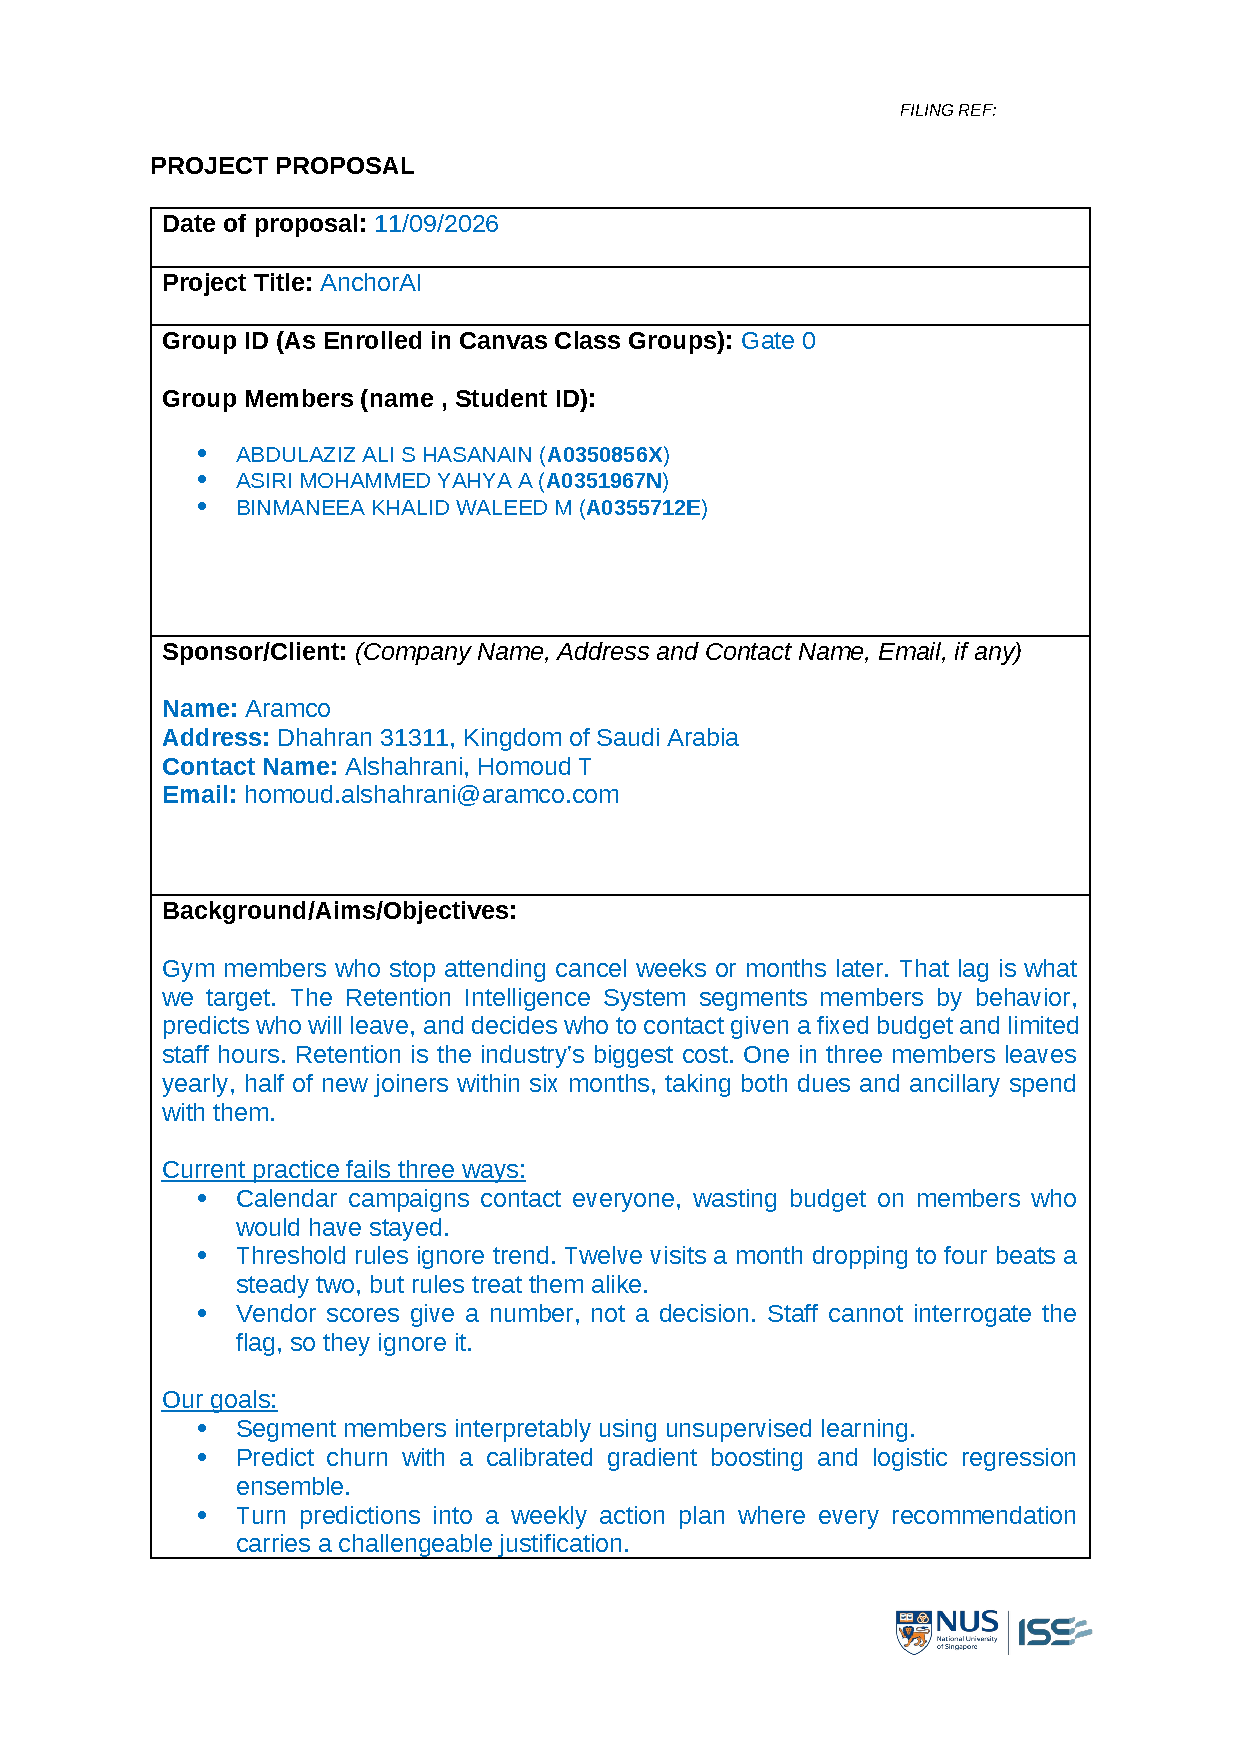
\includepdf[pages=1, scale=0.74, offset=0 -14mm, frame,
  pagecommand={\section{Project proposal}\label{app:proposal}\vspace{-0.4\baselineskip}{\small The proposal as submitted on 11 September 2026; pages 1--3 of the original, the fourth being blank.}}]{figures/appendix/proposal.pdf}
\includepdf[pages=2-3, scale=0.8, frame, pagecommand={\thispagestyle{scrheadings}}]{figures/appendix/proposal.pdf}

\section{Mapping to MR, RS and CGS}
\label{app:mapping}

All four technique groups the module requires are covered: decision automation, resource optimisation, knowledge discovery and cognitive systems (MR Machine Reasoning, RS Reasoning Systems, CGS Cognitive Systems; D is the course day). \Cref{tab:deviations} lists every change from the proposal and its reason.

% MR / RS / CGS mapping table, shared by both reports
{\small\sffamily
\begin{xltabular}{\linewidth}{@{}P{0.2\linewidth} L l P{0.2\linewidth}@{}}
  \caption{Techniques as built, by course and evidence.}\label{tab:mapping}\\
  \toprule
  \hd{Component} & \hd{Technique as built} & \hd{Course} & \hd{Evidence} \\
  \midrule
  \endfirsthead
  \toprule
  \hd{Component} & \hd{Technique as built} & \hd{Course} & \hd{Evidence} \\
  \midrule
  \endhead
  Data preparation & stratified split; SMOTE-NC inside folds compared with class weights; CRISP-DM & RS D2 & E2 \\
  Features & trend and ratio features, scaling, leakage check & MR D4, RS D2 & E2, leakage check \\
  Segmentation & K-means, silhouette, stability (adjusted Rand index), profiles & MR D4 & E1 \\
  Churn model & class-weighted logistic regression and LightGBM ensemble, Platt calibration; F1, PR-AUC, Brier & MR D2, D4 & E2 \\
  Driver explanations & averaged logistic-regression terms and TreeSHAP contributions per member & MR D3, D4 & E2 drivers \\
  Scenario layer & synthetic gym and randomised history with known effects & MR D3 & scenario layer \\
  Uplift baseline & T-learner (self-researched) & MR D4 & E3 \\
  Offer reasoner & case-based reasoning: retrieve, reuse, revise (shrinkage), retain & MR D2 & E3 \\
  Plan optimiser & genetic algorithm with repair, elitism, spillover and diminishing returns & RS D4 & E4, E5 \\
  Exact benchmark & CP-SAT constraint optimisation & MR D1, RS D1 & E5 \\
  Policy evaluation & simulation-based comparison against three baselines & RS D1 & E4 \\
  Rule engine & forward chaining over derive, playbook and guardrail rules; salience; traces; versions & MR D2, RS D1 & E6 \\
  Knowledge graph & Neo4j and Cypher; multi-hop cohort signals; read-only parameterised queries & MR D3, RS D5 & E7 \\
  Intent detection & sentence-embedding centroids with an unknown threshold; slot filling & CGS D1 & E8 \\
  Grounded generation & deterministic tool, then an LLM phrases cited evidence only & CGS D1, D3 & E8 \\
  Assistant evaluation & keyword baseline; static checks; calibrated LLM-as-judge; local and hosted models & CGS D2, D3 & E8 \\
  Message drafts & LLM drafts with a rule check and a template fallback & CGS D1 & drafts in the application \\
  Overall & hybrid machine learning, rules, optimisation, knowledge graph and language interface with human review & RS D1, CGS D1 & E4, E6, E7 \\
  \bottomrule
\end{xltabular}}


\clearpage
\subsection*{Deviations from the proposal}

{\small\sffamily
\begin{xltabular}{\linewidth}{@{}P{0.27\linewidth} P{0.27\linewidth} L@{}}
  \caption{Changes from the proposal and the presentation deck.}\label{tab:deviations}\\
  \toprule
  \hd{Proposal or deck} & \hd{Built} & \hd{Reason} \\
  \midrule
  \endfirsthead
  \toprule
  \hd{Proposal or deck} & \hd{Built} & \hd{Reason} \\
  \midrule
  \endhead
  A neural network picks who to contact (deck) & genetic algorithm, with CP-SAT as exact benchmark & a neural network learns; it cannot enforce budget or staff limits \\
  Agent-based longitudinal simulator & real Kaggle members plus a thin scenario layer & lower risk; segmentation and churn stay results on real data \\
  SMOTE to a 50/50 balance & SMOTE-NC inside folds compared with class weights; class weights kept; Platt calibration & oversampling inflates the probabilities the planner multiplies \\
  F1 and silhouette as the metrics & F1, PR-AUC, Brier, calibration and fairness gaps & the plan consumes probabilities \\
  Fuzzy inference for engagement tiers & not built & not taught in the three courses \\
  K-means and Gaussian mixture & K-means only & matches the deck and MR D4 \\
  CBR and uplift as separate components & CBR is the uplift estimator; the T-learner its benchmark & both estimate the same quantity \\
  Recency and regularity features; censoring & not built; censoring dropped & the snapshot has no visit dates and one binary label \\
  Exclude cancellation-process fields & a with-and-without check on same-month columns & the snapshot's leakage risk is timing \\
  Class recommendations; surrogate decision trees; graph embeddings & not built & stretch items \\
  Interviews with managers & simulated by an AI model, and disclosed & no real operator was reached \\
  The LLM calls tools itself & intent router before the LLM; tool calling optional & small local models are unreliable at tool calling \\
  \bottomrule
\end{xltabular}}

\clearpage
\section{Installation and user guide}
\label{app:install}

\paragraph{Install.} Prerequisites: Git, uv 0.13+, Node.js 20+, Docker with Compose, and optionally an OpenAI-compatible LLM endpoint (the default is a local Ollama \code{qwen2.5:7b-instruct}). Download \emph{Gym Customers Features and Churn} from Kaggle~\cite{vinueza-gym} into \code{SystemCode/data/raw/}; the data is CC BY-NC-SA 4.0 and not redistributed.
\begin{shell}
git clone <repo-url> AnchorAI && cd AnchorAI
cp .env.example .env                  # set ANCHORAI_JWT_SECRET and LLM_*
docker compose up -d neo4j            # knowledge graph
cd SystemCode/backend && uv sync
uv run anchorai setup                 # data, models, seeded DB, graph
uv run uvicorn anchorai.api.main:app  # API on :8000
cd ../frontend && npm install
npm run dev                           # web app on http://localhost:5173
\end{shell}
Sign in as \code{admin}, \code{manager}, \code{staff1} or \code{staff2} with the password \code{anchorai}. The pipeline, API and web application run without Neo4j or a language model, with the graph panels and assistant shown as unavailable. \code{uv run pytest -q} runs the 195 offline tests; \code{uv run anchorai db reset} restores the demo database; the administrator's Settings page checks every service.

\paragraph{Docker for everything.} Build the data on the host first, because the demo seed needs the tables; the API container migrates and seeds the database on start. Then load the graph from the host, or with \emph{Reload knowledge graph} on the Events \& roster page.
\begin{shell}
cd SystemCode/backend && uv sync && uv run anchorai data build
cd ../.. && docker compose up --build -d
cd SystemCode/backend && uv run anchorai kg load
\end{shell}

\begin{table}[!htb]
  \caption{Demo users. The password of every demo user is \code{anchorai}, or the value of \code{ANCHORAI_DEMO_PASSWORD}.}
  \label{tab:demousers}
  \begin{tabularx}{\linewidth}{@{}l l L@{}}
    \toprule
    \hd{User} & \hd{Role} & \hd{Lands on, and can use} \\
    \midrule
    \code{admin} & Admin & Dashboard; everything, including Rules, Offers \& constraints, Data \& models, Users, Audit log, Settings \\
    \code{manager} & Manager & Dashboard; Segments, Members, Weekly plan, Scenarios, Knowledge graph, Events \& roster \\
    \code{staff1}, \code{staff2} & Staff & My contacts; Member 360, Assistant \\
    \bottomrule
  \end{tabularx}
\end{table}

\paragraph{Checking the install.} In the application, the administrator's Settings page shows whether the language model, Neo4j, the models and the database are working, and tests the LLM connection.

\begin{table}[!htb]
  \caption{Troubleshooting.}
  \label{tab:trouble}
  \begin{tabularx}{\linewidth}{@{}P{0.42\linewidth} L@{}}
    \toprule
    \hd{Symptom} & \hd{Fix} \\
    \midrule
    \enquote{Expected exactly one Kaggle CSV} & put exactly one file, \code{gym_churn_us.csv}, in \code{SystemCode/data/raw/} \\
    Pages say the data tables are not built (HTTP 503) & run \code{uv run anchorai data build} \\
    Demo users cannot sign in & run \code{uv run anchorai db reset} \\
    Graph panels or assistant show \enquote{unavailable} & start Neo4j or the LLM endpoint; the rest keeps working \\
    \code{npm} fails with an engine or native-binding error & upgrade to Node 20 or newer, delete \code{node_modules} and reinstall \\
    Docker reports a missing host--sandbox network interface & the kernel was updated without a reboot; reboot \\
    Port 8000 or 5173 is in use & stop the other process, or change the port \\
    \bottomrule
  \end{tabularx}
\end{table}

\paragraph{Using the application.} AnchorAI has three roles, and the role decides which pages appear in the sidebar; the server checks the role again on every request. A session lasts 12 hours. Every page has a member search at the top (Ctrl+K), a light, dark or system theme, and, except on the Assistant page itself, a round button that opens the assistant beside the current page.

\paragraph{Manager: check the risk.} The \emph{Dashboard} (\cref{fig:screens}) shows members at high risk (a churn probability of 0.6 or more), the monthly revenue at risk (the sum of churn probability × monthly fee), the share of high-risk members covered by the latest approved plan, the latest week's contacted, reached and retained counts, the risk distribution, the segment mix and outcomes by week. \emph{Segments} shows one card per segment with its size, churn rate, members at high risk now, revenue and a profile against all members. \emph{Members} filters by ID, segment, risk band, club and tenure, sorts by any column and exports every matching member to CSV. A row opens \emph{Member 360}.

\paragraph{Manager: build, review and approve the plan.} On \emph{Weekly plan} (\cref{fig:screens}), enter the weekly budget and staff hours (they start from the latest plan, or \$1,500 and 36 hours), choose a planner (the genetic algorithm by default, which considers members who train together; exact; or greedy, the quickest) and select \emph{Generate plan}. Four tiles sum it up: members to contact, spend, staff time and extra members expected to stay, each compared with last week. \emph{Why} on a row opens the member's summary, churn drivers, the rules that fired, any gym events and the ten most similar past members with what happened to them. While the plan is a draft you can remove a member, add a contact or swap an offer; each change needs a reason and is checked against the rules at once (red: blocked, with the rule; amber: allowed but not proposed by a playbook; green: allowed and proposed). \emph{Re-optimise the rest} keeps your changes and re-plans what is left of the budget, staff time and stock. \emph{Approve plan} locks it; only one plan per week can be approved. Contacts are then shared out, most valuable first, to the staff member with the most free time who has the right skill. Drag a contact to another staff member, re-run the assignment, and print or download each person's call sheet.

\paragraph{Manager: what-ifs and events.} \emph{Scenarios} (\cref{fig:ug}a) runs five planners (contact everyone, riskiest first, greedy, exact and the genetic algorithm) on the same week at a budget and staff hours you choose, compares contacts, spend, staff time, extra members, members per \$1,000 and per staff hour, and saves named comparisons. Nothing here changes the plan. On \emph{Events \& roster}, record what really happened: add instructors and classes, change who teaches a class, mark an instructor as left or a class as cancelled for a given week, or reinstate them. The graph is rebuilt after each change, and rules that read graph signals then fire for the affected members; churn scores do not change. On \emph{Knowledge graph} (\cref{fig:kgsim}), simulate an instructor leaving or a class closing to see who would be affected, how many are high risk and which rules would newly fire, without changing anything.

\begin{figure}[!htb]
  \centering
  \begin{subfigure}[t]{0.328\linewidth}
    \screenshot[\linewidth]{screens/scenarios-content.png}
    \caption{Scenarios: set a week's budget and staff hours and compare five planners side by side.}
  \end{subfigure}\hfill
  \begin{subfigure}[t]{0.328\linewidth}
    \screenshot[\linewidth]{screens/my-contacts-done-content.png}
    \caption{My contacts: the staff call list with outcomes logged.}
  \end{subfigure}\hfill
  \begin{subfigure}[t]{0.328\linewidth}
    \screenshot[\linewidth]{screens/rules-test-content.png}
    \caption{Rules: testing the rule base on one member shows the same trace as Member 360.}
    \label{fig:rulestrace}
  \end{subfigure}
  \caption{One page for each role: manager, staff and administrator.}
  \label{fig:ug}
\end{figure}

\paragraph{Staff: contacts, drafts and the assistant.} \emph{My contacts} (\cref{fig:ug}b) lists the members assigned to you in this week's approved plan, highest priority first, each with the offer and channel, why the member is on the list, talking points from their risk drivers and the rule that proposed the offer. Log an outcome in two taps: \emph{Accepted}, \emph{Declined}, \emph{Reached} (no decision yet), \emph{Follow-up} or \emph{No answer}, optionally with a note. Accepted and declined outcomes become new past cases, and every logged contact counts towards the contact limits, so the member is not contacted again too soon. \emph{Draft message}, next to an allowed offer in a member's rule trace, writes a short SMS, email, call script or in-person note that you edit and copy into your own tool; AnchorAI never sends anything, and a draft never mentions churn, risk or scores. In the \emph{Assistant} (\cref{fig:assistant}), type a question and press Enter. It answers about member risk, what to offer, comparisons, ranked lists, who an event affects and, for managers, the plan and what-if budgets or staff hours, always from AnchorAI's own data. Numbers in an answer are chips that show the evidence behind each sentence. When nothing supports an answer it says \enquote{I don't know based on the data I have}. It cannot change anything and does not remember a conversation after a refresh.

\paragraph{Administrator.} The \emph{Rules} page (\cref{fig:ug}c) lists every rule with its kind, salience, conditions, action and source, under a validation banner. Toggle a rule on or off, add or edit one in a form that validates as you type, or edit the YAML directly; every save needs a note and creates a new version, and nothing is overwritten. \emph{Test on a member} runs the saved rules, or an unsaved draft, on any member and shows the same trace as Member~360. \emph{Versions} compares any two versions line by line and rolls back to an older one. \emph{Offers \& constraints} edits the offer catalogue (cost, staff time, stock, channels, required skill, eligibility, active), each staff member's weekly hours and skills, and the planning defaults: weekly budget, staff minutes and the contact caps the guardrails read. \emph{Data \& models} replaces the source file with a validated new Kaggle file, rebuilds data and models with any seed in the background (42 reproduces this report), reloads the graph, and shows the model card. \emph{Users} creates accounts, changes roles and deactivates users; \emph{Audit log} records every write with who, when, and the values before and after; \emph{Settings} is a read-only health check of the language model, the knowledge graph, the models and data, and the database.

\begingroup\let\chapter\section
\chapter{Use of AI tools}
\label{app:aiuse}

\paragraph{AI tool declaration.} We used Claude Code to help plan the project, write, review and test code, run and check experiments, draft and edit report text, and build the slide decks and editing scripts for the videos. We are responsible for the content and quality of the submitted work.

The team used an AI coding assistant (Claude Code) throughout and logged every meaningful use in the repository, with what it was used for and how the result was checked; the log is reproduced below. Three principles applied. Every output was reviewed by the member responsible, and every number in this report was re-measured against the committed results and notebooks rather than taken from the tool. Design decisions, such as the choice of estimator, planner defaults and experiment axes, were made by the team. And where AI stood in for people, it is disclosed: the manager interviews that shaped the rule base were simulated by an AI model and are treated as plausible opinion, not evidence (\cref{sec:acquisition}); 62 of the assistant's 86 test questions were AI-written and are reported separately from the 24 written by team members (E8). The report text was drafted with AI assistance from the team's own section drafts and reviewed by the team. No AI-generated speech is used in the videos. In the log, Abdulaziz is Abdulaziz Ali S Hasanain, Asiri is Asiri Mohammed Yahya A, and Mokdy is Binmaneea Khalid Waleed M.

{\small\sffamily
\begin{xltabular}{\linewidth}{@{}l l P{0.36\linewidth} L@{}}
  \caption{The AI-use log, generated from \code{docs/AI_USE.md}; the tool in every row is Claude Code.}\label{tab:aiuse}\\
  \toprule
  \hd{Date} & \hd{Member} & \hd{Used for} & \hd{What we changed or verified} \\
  \midrule
  \endfirsthead
  \toprule
  \hd{Date} & \hd{Member} & \hd{Used for} & \hd{What we changed or verified} \\
  \midrule
  \endhead
  \csname @@input\endcsname appendices/f-ai-use-rows.tex 
  \bottomrule
\end{xltabular}}

\endgroup

\clearpage
\section{Individual project reports}
\label{app:reflections}
% Individual project report pages, shared by both reports: one page per member with their reflection.
% Each member writes appendices/reflection-<key>.tex. Peer reviews are confidential and built separately (ProjectReport/peer-review/).
% #1 sectioning level (section or subsection), #2 member's name, #3 file key
\newcommand{\individualreport}[3]{%
  \csname #1\endcsname*{#2}\addcontentsline{toc}{#1}{#2}
  \minisec{\color{nusBlue}Individual reflection}
  \InputIfFileExists{appendices/reflection-#3}{}{\emph{To be written by #2.}}\par
  \clearpage}

\individualreport{subsection}{Abdulaziz Ali S Hasanain}{abdulaziz}
\individualreport{subsection}{Asiri Mohammed Yahya A}{asiri}
\individualreport{subsection}{Binmaneea Khalid Waleed M}{khalid}

\end{document}
